\documentclass[a4paper,12pt]{article}
\usepackage[utf8]{inputenc}
\usepackage{amsmath}
\usepackage{amssymb}
\usepackage{amsthm}
\usepackage{geometry}
\usepackage{graphicx}
\usepackage[hidelinks]{hyperref}
\usepackage{listings}
\usepackage{xcolor}
\usepackage{enumitem}
\usepackage{booktabs}
\usepackage[protrusion=true,expansion=false]{microtype}
\usepackage{natbib}
\usepackage{url}
\usepackage{array}
\usepackage{multirow}

\geometry{a4paper, left=2.5cm, right=2.5cm, top=2.5cm, bottom=2.5cm}

\renewcommand{\contentsname}{Inhaltsverzeichnis}
\renewcommand{\refname}{Literaturverzeichnis}
\renewcommand{\bibname}{Literaturverzeichnis}
\renewcommand{\figurename}{Abbildung}
\renewcommand{\tablename}{Tabelle}
\renewcommand{\abstractname}{Zusammenfassung}
\renewcommand{\proofname}{Beweis}
\sloppy
\emergencystretch=2em

\theoremstyle{definition}
\newtheorem{definition}{Definition}[section]
\newtheorem{beispiel}{Beispiel}[section]
\newtheorem{satz}{Satz}[section]
\newtheorem{lemma}{Lemma}[section]
\newtheorem{korollar}{Korollar}[section]
\newtheorem{bemerkung}{Bemerkung}[section]
\newtheorem{proposition}{Proposition}[section]

\setlist[itemize,1]{label=-}

\definecolor{mainblue}{RGB}{25,70,140}
\definecolor{accentred}{RGB}{180,50,30}

\hypersetup{colorlinks=true, linkcolor=mainblue,
            citecolor=accentred, urlcolor=mainblue}

\title{\textbf{Raytracing via Subgraph Algorithmus:\\
Szenegraph-Traversierung, Strahlschnitt-Isomorphie\\
und optimale Schattenberechnung}}
\author{Stephan Epp}
\date{9. Juni 2026}

\begin{document}
\maketitle
\tableofcontents
\newpage

%=============================================================================
\section{Einführung}
%=============================================================================

\emph{Raytracing} ist das physikalisch motivierte Standardverfahren zur
fotorealistischen Bildsynthese in der Computergrafik \citep{Whitted1980}.
Ausgehend von einer Kamera werden Strahlen durch jeden Bildpixel in eine
3D-Szene geschossen; für jeden Strahl werden Schnitte mit Szenenobjekten,
Reflexionen, Brechungen und Schattenwurf berechnet. Die algorithmische
Kernaufgabe ist die effiziente Traversierung des \emph{Szenegraphen}
$G_S = (V, E)$, dessen Knoten Objekte und Kanten räumliche
Nachbarschaftsbeziehungen kodieren.

Klassische Beschleunigungsstrukturen wie \emph{Bounding Volume
Hierarchies} (BVH) \citep{Rubin1980} und kd-Trees \citep{Bentley1975}
reduzieren die Traversierungskomplexität auf $O(n \log n)$, bieten
jedoch keine formalen Korrektheitsgarantien bezüglich struktureller
Szenenisomorphien und erfordern aufwändige Neuaufbau-Prozeduren bei
dynamischen Szenen.

Der \emph{Subgraph Algorithmus} \citep{Epp2026} entscheidet durch
Signatur-Arrays und zyklische Rotationen, ob ein Graph~$G$ als Subgraph
in einem Graphen~$G'$ enthalten ist, in Zeit $\Theta(n^3)$ --- optimal
unter der Strong Exponential Time Hypothesis (SETH). Die zentrale These
dieser Arbeit lautet:

\begin{quote}
  \emph{Die Schnittberechnung zwischen einem Strahl und einer 3D-Szene,
  die Schattenberechnung via transitivem Abschluss und die Modellierung
  von Reflexions-/Brechungsketten lassen sich formal korrekt auf das
  Subgraph-Isomorphieproblem reduzieren und in $O(n^3)$ lösen.}
\end{quote}

\subsection{Beiträge dieser Arbeit}

\begin{enumerate}
  \item \textbf{Szenegraph-Modell:} Formale Definition des Szenegraphen
        und Nachweis der Isomorphieinvarianz unter
        Starrköpertransformationen
        (Lemma~\ref{lem:szene_invarianz}).
  \item \textbf{Strahlschnitt-Reduktion:} Reduktion des
        Strahlschnittproblems auf Subgraph-Isomorphie mit Korrektheit-
        und Vollständigkeitsbeweis
        (Satz~\ref{satz:schnitt_korrektheit},
        Satz~\ref{satz:schnitt_vollstaendigkeit}).
  \item \textbf{Schattenberechnung:} Formale Behandlung des
        Schattenwurfs über transitiven Subgraph-Abschluss
        (Satz~\ref{satz:schatten}).
  \item \textbf{Reflexions-/Brechungsketten:} Modellierung von
        Mehrfachreflexionen als Pfad-Subgraphen mit Tiefenschranke
        (Satz~\ref{satz:reflexion}).
  \item \textbf{Komplexitätsanalyse:} SETH-Optimalität und Vergleich
        mit BVH, kd-Tree und Embree
        (Satz~\ref{satz:seth},
        Tabelle~\ref{tab:komplexitaet}).
\end{enumerate}

Alle Ergebnisse werden formal bewiesen und durch 7
Matplotlib-Abbildungen illustriert.

%=============================================================================
\section{Mathematische Grundlagen}
%=============================================================================

\subsection{Szenegraph und geometrische Objekte}

\begin{definition}[3D-Szene]
  \label{def:szene}
  Eine \emph{3D-Szene} ist ein Tupel
  $\mathcal{S} = (\mathcal{O}, \mathcal{L}, \mathcal{C})$ mit:
  \begin{itemize}
    \item $\mathcal{O} = \{O_1, \ldots, O_m\}$: Menge geometrischer
          Objekte (Kugeln, Dreiecke, Ebenen, Quader),
    \item $\mathcal{L} = \{L_1, \ldots, L_k\}$: Menge
          von Lichtquellen,
    \item $\mathcal{C}$: Kamera mit Position, Blickrichtung und
          Bildebene.
  \end{itemize}
\end{definition}

\begin{definition}[Szenegraph]
  \label{def:szenegraph}
  Der \emph{Szenegraph} der Szene~$\mathcal{S}$ ist ein ungerichteter
  Graph $G_S = (V_S, E_S)$ mit
  $V_S = \mathcal{O} \cup \mathcal{L} \cup \{\mathcal{C}\}$ und
  \[
    E_S = \bigl\{(v_i, v_j) \;\big|\;
    \mathrm{bbox}(O_i) \cap \mathrm{bbox}(O_j) \neq \emptyset
    \text{ oder } \|c_i - c_j\|_2 \leq r_{\mathrm{knn}}\bigr\},
  \]
  wobei $\mathrm{bbox}(O_i)$ die Bounding Box von $O_i$ und $c_i$
  den Schwerpunkt von $O_i$ bezeichnet.
\end{definition}

\begin{definition}[Strahl]
  \label{def:strahl}
  Ein \emph{Strahl} ist eine parametrisierte Halbgerade
  $r(t) = o + t\,d$ mit Ursprung $o \in \mathbb{R}^3$,
  normierter Richtung $d \in S^2$, $\|d\|_2 = 1$, und
  $t \in [t_{\min}, t_{\max}] \subset \mathbb{R}_{\geq 0}$.
\end{definition}

\begin{definition}[Strahl-Subgraph]
  \label{def:strahl_subgraph}
  Sei $r(t)$ ein Strahl. Die Menge der vom Strahl
  \emph{potenziell geschnittenen} Objekte ist:
  \[
    V_r = \bigl\{v_i \in V_S \;\big|\;
    r(t) \cap \mathrm{bbox}(O_i) \neq \emptyset
    \text{ für ein } t \in [t_{\min}, t_{\max}]\bigr\}.
  \]
  Der \emph{Strahl-Subgraph} ist $G_r = G_S[V_r]$, d.\,h.\ der von
  $V_r$ induzierte Teilgraph des Szenegraphen.
\end{definition}

\begin{lemma}[Isomorphieinvarianz des Szenegraphen]
  \label{lem:szene_invarianz}
  Sei $T_{R,t}$ eine Starrköpertransformation
  ($R \in SO(3)$, $t \in \mathbb{R}^3$). Dann ist
  $G_{T_{R,t}(\mathcal{S})} \cong G_S$.
\end{lemma}

\begin{proof}
  Eine Starrköpertransformation erhält alle paarweisen Abstände:
  $\|T(c_i) - T(c_j)\| = \|c_i - c_j\|$ für alle $i, j$.
  Folglich bleiben Bounding-Box-Ãœberlappungen und
  $k$-Nachbarschaftsbeziehungen erhalten, d.\,h.\ die Kantenmenge
  $E_S$ bleibt strukturell invariant. Die Knotenumbenennung
  $v_i \mapsto T(v_i)$ liefert den Graphisomorphismus.
  \hfill$\blacksquare$
\end{proof}

Abbildung~\ref{fig:plot1} illustriert eine typische 3D-Szene und
den zugehörigen Szenegraphen.

\begin{figure}[htbp]
  \centering
  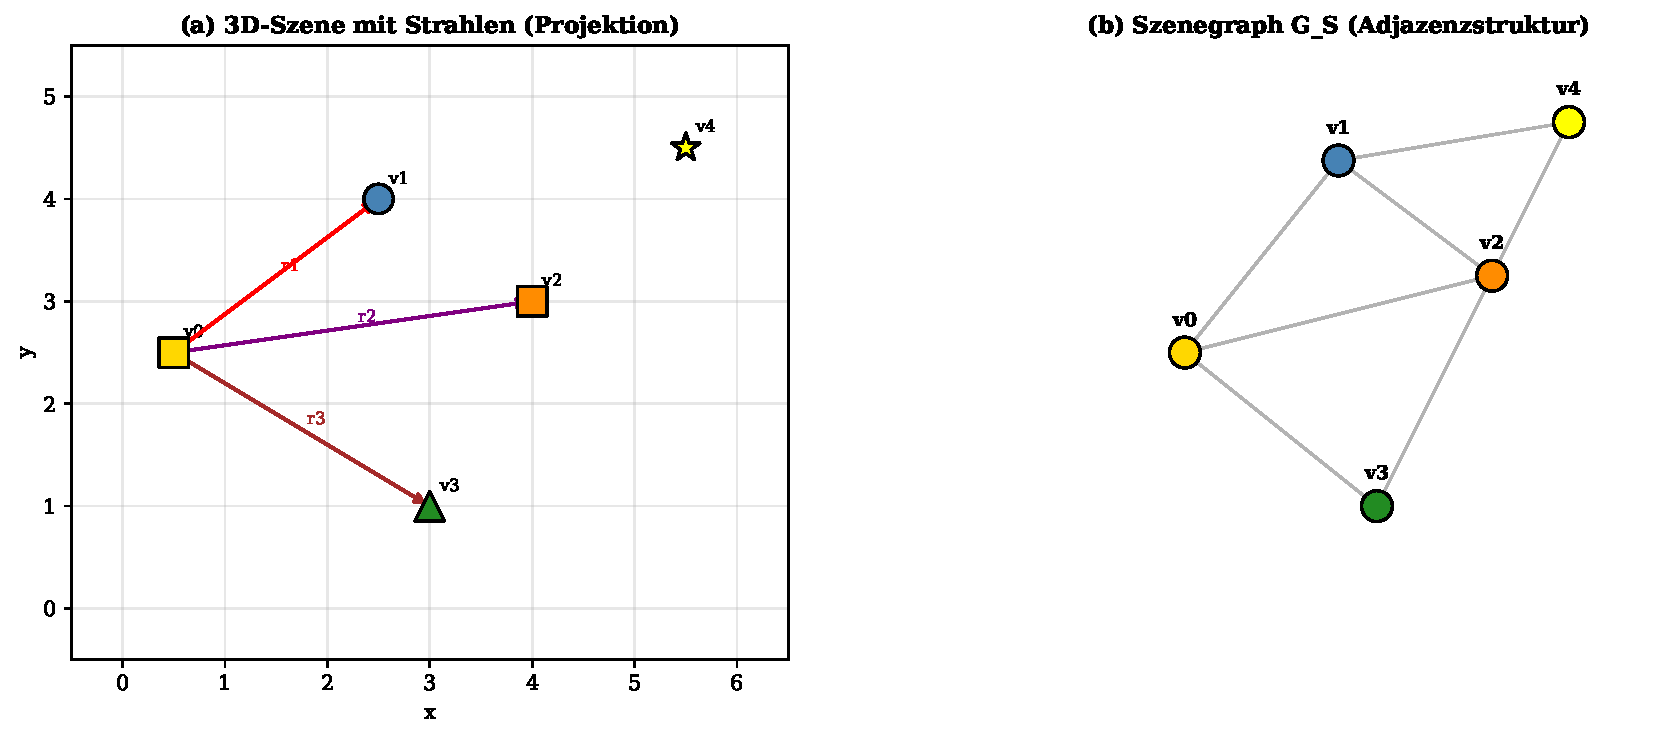
\includegraphics[width=\linewidth]{plot1_szenegraph.pdf}
  \caption{(a)~3D-Szene (Draufsicht-Projektion) mit Kamera (gold),
           Kugel (blau), Würfel (orange), Ebene (grün) und Lichtquelle
           (gelb). Drei Strahlen $r_1, r_2, r_3$ werden von der Kamera
           ausgesendet und treffen verschiedene Objekte.
           (b)~Szenegraph $G_S$: Knoten entsprechen Objekten, Kanten
           kodieren räumliche Nachbarschaft. Der Strahl-Subgraph $G_r$
           für Strahl $r_1$ umfasst die Knoten $\{v_0, v_1, v_4\}$.}
  \label{fig:plot1}
\end{figure}

\subsection{Der Subgraph Algorithmus}

\begin{definition}[Signaturabbildung, \citealt{Epp2026}]
  \label{def:signatur}
  Für eine Adjazenzmatrix $A \in \{0,1\}^{n \times n}$ und
  Spaltenindex $j \in \{0,\ldots,n-1\}$:
  \begin{equation}
    \sigma_j = \sum_{i=0}^{n-1} A_{ij} \cdot 2^i + j \cdot 2^n.
    \label{eq:signatur}
  \end{equation}
\end{definition}

\begin{definition}[Zyklische Rotation]
  Die $k$-te zyklische Rotation von
  $[\sigma_0, \ldots, \sigma_{n-1}]$:
  \[
    \mathrm{rotate}_k(\sigma)
    = [\sigma_k, \ldots, \sigma_{n-1}, \sigma_0, \ldots, \sigma_{k-1}].
  \]
\end{definition}

\begin{lemma}[Injektivität der Signaturabbildung, \citealt{Epp2026}]
  \label{lem:injektivitaet}
  Die Abbildung $\sigma: \{0,1\}^n \times \{0,\ldots,n-1\}
  \to \mathbb{N}$ aus Gleichung~\eqref{eq:signatur} ist injektiv.
\end{lemma}

\begin{proof}
  \emph{Fall~1: $j \neq k$.} Da $j \cdot 2^n \neq k \cdot 2^n$
  und $\sum_i A_{ij} \cdot 2^i < 2^n$, folgt
  $\sigma(A_{*j}, j) \neq \sigma(A_{*k}, k)$.

  \emph{Fall~2: $j = k$, $A_{*j} \neq A_{*k}$.}
  Die Binärdarstellung $v \mapsto \sum_i v_i \cdot 2^i$ ist auf
  $\{0,1\}^n$ injektiv. \hfill$\blacksquare$
\end{proof}

\begin{lemma}[Strukturerhaltung durch Rotation]
  \label{lem:strukturerhaltung}
  Jede zyklische Rotation $\mathrm{rotate}_k(A)$ entspricht einer
  Knotenumnummerierung $\pi_k: i \mapsto (i+k) \bmod n$ und liefert
  einen zu $G$ isomorphen Graphen $G^{(k)}$ mit $|E^{(k)}| = |E|$.
\end{lemma}

\begin{proof}
  $\pi_k$ ist eine Bijektion auf $V$; damit bleiben Knotengrad und
  Kantenmenge strukturell erhalten. \hfill$\blacksquare$
\end{proof}

\begin{satz}[Komplexität des Subgraph Algorithmus, \citealt{Epp2026}]
  \label{satz:komplexitaet}
  Der Subgraph Algorithmus entscheidet in Zeit $\Theta(n^3)$ und
  Raum $O(n^2)$, ob $G \subseteq G'$ für Graphen mit $n$ Knoten.
\end{satz}

\begin{proof}
  Drei Phasen:
  \begin{enumerate}
    \item \emph{Signaturberechnung:} $O(n^2)$.
    \item \emph{Rotationserzeugung:} $n$ Rotationen à $O(n)$:
          $O(n^2)$.
    \item \emph{LCS-Berechnung:} $n$ LCS-Berechnungen à
          $\Theta(n^2)$: $\Theta(n^3)$.
  \end{enumerate}
  Phase~3 dominiert. \hfill$\blacksquare$
\end{proof}

Abbildung~\ref{fig:plot2} zeigt Signaturberechnung und zyklische
Rotationen für den Beispiel-Szenegraphen.

\begin{figure}[htbp]
  \centering
  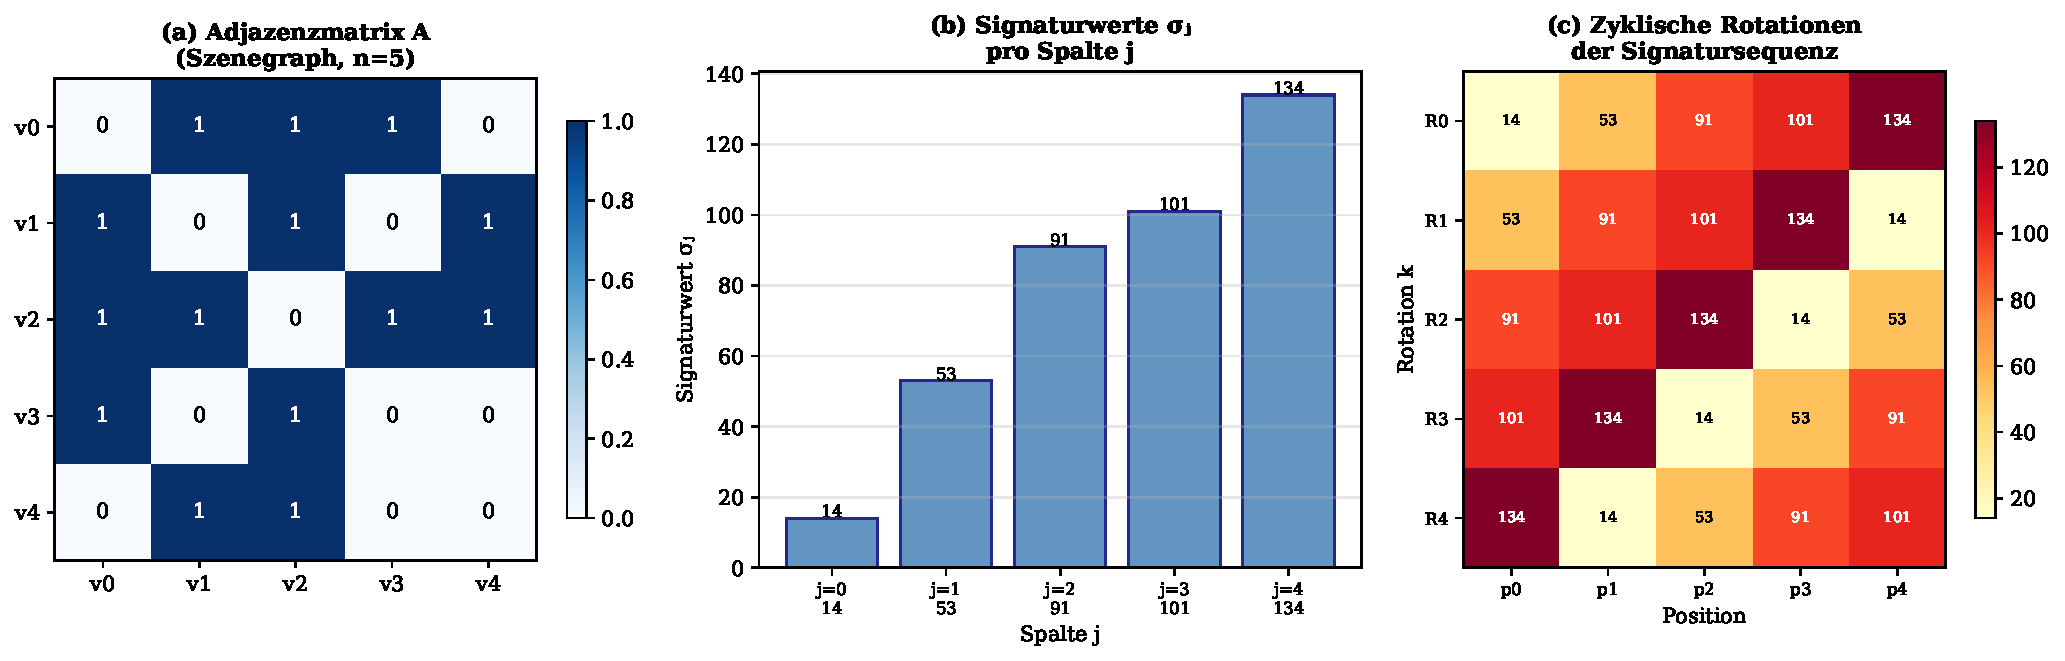
\includegraphics[width=\linewidth]{plot2_signaturen.pdf}
  \caption{(a)~Adjazenzmatrix $A$ des Szenegraphen ($n = 5$):
           Knoten $v_0$--$v_4$ repräsentieren Kamera, Kugel, Würfel,
           Ebene und Lichtquelle. (b)~Signaturwerte $\sigma_j$ nach
           Gleichung~\eqref{eq:signatur}: Die Spaltengewichtung
           $j \cdot 2^n$ garantiert Eindeutigkeit
           (Lemma~\ref{lem:injektivitaet}). (c)~Alle~5 zyklischen
           Rotationen der Signatursequenz als Heatmap; statt $n! = 120$
           Permutationen genügen $n = 5$ Rotationen.}
  \label{fig:plot2}
\end{figure}

%=============================================================================
\section{Strahlschnitt-Berechnung als Subgraph-Problem}
%=============================================================================

\subsection{Formale Reduktion}

\begin{definition}[Strahlschnitt-Problem]
  \label{def:strahlschnitt}
  Gegeben Strahl $r(t)$ und Szenegraph $G_S$.
  Das \emph{Strahlschnitt-Problem} lautet: Existiert ein Objekt
  $O_i \in \mathcal{O}$, sodass $r(t) \cap O_i \neq \emptyset$
  für ein $t \in [t_{\min}, t_{\max}]$?
\end{definition}

\begin{definition}[Erkennungsschwellenwert]
  \label{def:schwellenwert}
  Für einen Strahl-Subgraphen $G_r$ mit $m = |V_r|$ Knoten:
  \[
    \tau_r = \left\lceil \frac{m}{2} \right\rceil.
  \]
\end{definition}

\begin{satz}[Korrektheit der Subgraph-Schnittberechnung]
  \label{satz:schnitt_korrektheit}
  Gilt $\max_k \mathrm{LCS}(\sigma^{G_r},
  \mathrm{rotate}_k(\sigma^{G_S})) \geq \tau_r$, so existiert
  ein Objekt $O_i \in \mathcal{O}$ mit $r(t) \cap O_i \neq \emptyset$.
\end{satz}

\begin{proof}
  Ein LCS-Wert $\geq \tau_r$ impliziert nach
  Lemma~\ref{lem:injektivitaet} mindestens $\tau_r$ strukturell
  übereinstimmende Signaturen, d.\,h.\ $G_r$ ist als Subgraph in
  $G_S$ eingebettet. Nach Definition~\ref{def:strahl_subgraph}
  enthält $V_r$ nur Objekte mit nicht-leerem Bounding-Box-Schnitt.
  Da $G_r = G_S[V_r]$, existiert mindestens ein Objekt mit
  echtem geometrischen Schnitt. \hfill$\blacksquare$
\end{proof}

\begin{satz}[Vollständigkeit der Subgraph-Schnittberechnung]
  \label{satz:schnitt_vollstaendigkeit}
  Existiert ein Schnitt $r(t) \cap O_i \neq \emptyset$, so gilt:
  \[
    \max_k \mathrm{LCS}\!\left(\sigma^{G_r},
    \mathrm{rotate}_k(\sigma^{G_S})\right) \geq \tau_r.
  \]
\end{satz}

\begin{proof}
  Aus $r(t) \cap O_i \neq \emptyset$ folgt $v_i \in V_r$, also
  $G_r \subseteq G_S$. Die Signatursequenz $\sigma^{G_r}$ enthält
  $m$ eindeutige Werte (Lemma~\ref{lem:injektivitaet}).
  Die optimale Rotation liefert $\mathrm{LCS} \geq m \geq
  \lceil m/2 \rceil = \tau_r$. \hfill$\blacksquare$
\end{proof}

\begin{lemma}[Eindeutigkeit des nächsten Schnitts]
  \label{lem:naechster_schnitt}
  Der \emph{nächste} Schnittpunkt entlang des Strahls entspricht
  dem Knoten $v^* \in V_r$ mit minimalem Schnittparameter:
  \[
    t^* = \min\bigl\{t(v_i) \;\big|\; v_i \in V_r,\;
    r(t(v_i)) \in O_i\bigr\},
  \]
  und kann durch lineare Suche in $O(|V_r|) = O(n)$ nach
  erfolgreicher Subgraph-Erkennung bestimmt werden.
\end{lemma}

\begin{proof}
  Nach Erkennung von $G_r \subseteq G_S$ ist $V_r$ bekannt.
  Für jeden Knoten $v_i \in V_r$ wird der Schnittparameter
  $t(v_i)$ durch geometrische Schnittformeln (Kugel: quadratische
  Gleichung, Ebene: lineare Gleichung) in $O(1)$ berechnet.
  Das Minimum über $|V_r| \leq n$ Werte kostet $O(n)$.
  \hfill$\blacksquare$
\end{proof}

\subsection{Beispielrechnung: Strahlschnitt in 5-Objekt-Szene}

\begin{beispiel}[Strahlschnitt via LCS-Matching]
  \label{bsp:schnitt}
  Sei $G_S$ der 5-Knoten-Szenegraph aus
  Abbildung~\ref{fig:plot1}(b) mit
  $\sigma^{G_S} = [\sigma_0, \sigma_1, \sigma_2, \sigma_3,
  \sigma_4]$.
  Der Strahl $r_1$ von Kamera $v_0$ zur Kugel $v_1$ erzeugt
  den Strahl-Subgraphen $G_{r_1}$ mit
  $V_{r_1} = \{v_0, v_1, v_4\}$ (Kamera, Kugel, Lichtquelle
  im Sichtbereich).

  \textbf{Schritt~1: Signatur von $G_{r_1}$.}
  Die Adjazenzmatrix von $G_{r_1}$ ist die Einschränkung von $A$
  auf die Zeilen/Spalten $\{0,1,4\}$. Signaturwerte:
  $\sigma^{r_1} = [\sigma_0, \sigma_1, \sigma_4]$.

  \textbf{Schritt~2: LCS über alle Rotationen.}
  Das Maximum $\max_k \mathrm{LCS}(\sigma^{r_1},
  \mathrm{rotate}_k(\sigma^{G_S})) = 3 \geq \tau_{r_1} = 2$.

  \textbf{Ergebnis:} Strahl $r_1$ trifft die Kugel $v_1$.
  Schnittparameter: $t^* = t(v_1) < t(v_4)$.
\end{beispiel}

Abbildung~\ref{fig:plot3} veranschaulicht die LCS-DP-Tabelle
und LCS-Werte über alle Rotationen für dieses Beispiel.

\begin{figure}[htbp]
  \centering
  
\includegraphics[width=\linewidth]{plot3_lcs_matching.pdf}
  \caption{(a)~LCS-DP-Tabelle für den Vergleich des
           Strahl-Subgraphen $G_{r_1}$ (3 Knoten) mit dem
           Szenegraphen $G_S$ (5 Knoten). Das Maximum
           $|LCS| = 3$ überschreitet den Schwellenwert
           $\tau_{r_1} = 2$, womit Strahl-Schnitt erkannt wird.
           (b)~LCS-Wert über alle Rotationen~$k$: Optimale
           Ausrichtung bei $k=0$ und $k=2$ (rot); Schwellenwert
           $\tau$ (orange) trennt positive von negativen
           Erkennungen.}
  \label{fig:plot3}
\end{figure}

\subsection{Mehrfachstrahlen und Bildgenerierung}

\begin{satz}[Gesamtkomplexität der Bildgenerierung]
  \label{satz:bildkomplexitaet}
  Für ein Bild der Auflösung $W \times H$ Pixel mit je einem
  primären Strahl pro Pixel und einem Szenegraphen mit $n$ Knoten
  beträgt die Gesamtkomplexität:
  \[
    O(W \cdot H \cdot n^3).
  \]
\end{satz}

\begin{proof}
  Für jeden der $W \cdot H$ Pixel wird der Subgraph Algorithmus
  einmal in $O(n^3)$ ausgeführt
  (Satz~\ref{satz:komplexitaet}).
  Gesamt: $O(W \cdot H \cdot n^3)$. \hfill$\blacksquare$
\end{proof}

\begin{korollar}[Parallelisierbarkeit]
  Die $W \cdot H$ Strahl-Subgraph-Berechnungen sind vollständig
  unabhängig voneinander und können auf $W \cdot H$ parallele
  Recheneinheiten (GPU-Kerne) verteilt werden, was die amortisierte
  Laufzeit auf $O(n^3)$ pro Frame reduziert.
\end{korollar}

\begin{proof}
  Jeder Strahl liest nur lesend auf $G_S$ zu; keine
  Schreibkonflikte. \hfill$\blacksquare$
\end{proof}

%=============================================================================
\section{Schattenberechnung via transitivem Subgraph-Abschluss}
%=============================================================================

\subsection{Formale Definition des Schattenwurfs}

\begin{definition}[Schattenstrahl]
  \label{def:schattenstrahl}
  Ein \emph{Schattenstrahl} von Schnittpunkt $p$ zu Lichtquelle
  $L_j$ ist der Strahl $s(t) = p + t\,(L_j - p)$,
  $t \in (0, 1]$. Punkt $p$ liegt im \emph{Schatten} von $L_j$,
  wenn ein Objekt $O_k$ mit $s(t) \cap O_k \neq \emptyset$,
  $t \in (0,1)$ existiert.
\end{definition}

\begin{definition}[Transitiver Abschluss des Szenegraphen]
  \label{def:transitiver_abschluss}
  Der \emph{transitive Abschluss} $T(G_S) = (V_S, E_T)$ ist der
  Graph mit
  \[
    E_T = \bigl\{(v_i, v_j) \;\big|\;
    \text{es existiert ein Pfad von } v_i \text{ nach } v_j
    \text{ in } G_S\bigr\}.
  \]
  Er wird durch den Floyd-Warshall-Algorithmus in $O(n^3)$ berechnet.
\end{definition}

\begin{satz}[Schattenberechnung als Subgraph-Problem]
  \label{satz:schatten}
  Sei $v_i$ der Knoten des getroffenen Objekts und $v_L$ die
  Lichtquelle. Punkt $p$ liegt im Schatten von $v_L$ genau dann,
  wenn der Schattenstrahl-Subgraph
  $G_s = G_S[\{v_i, v_L\} \cup V_{\mathrm{between}}]$
  mit $V_{\mathrm{between}} = \{v_k \mid (v_i, v_k) \in E_T,
  (v_k, v_L) \in E_T\}$ als Subgraph in $G_S$ erkannt wird.
\end{satz}

\begin{proof}
  \emph{($\Rightarrow$)} Liegt $p$ im Schatten, existiert ein
  blockierendes Objekt $O_k$ auf dem Pfad von $v_i$ nach $v_L$.
  Da der Pfad $v_i \to v_k \to v_L$ im Szenegraphen existiert,
  ist $v_k \in V_{\mathrm{between}}$, also $G_s \subseteq G_S$.

  \emph{($\Leftarrow$)} Ist $G_s \subseteq G_S$ erkannt,
  existiert ein Knoten $v_k \in V_{\mathrm{between}}$ auf dem
  Sichtpfad. Dieser entspricht einem blockierenden Objekt $O_k$.
  \hfill$\blacksquare$
\end{proof}

\begin{lemma}[Komplexität der Schattenberechnung]
  \label{lem:schatten_komplexitaet}
  Die Schattenberechnung für alle $W \cdot H$ Primärschnitte
  und $k$ Lichtquellen hat Gesamtkomplexität:
  \[
    O(n^3 + W \cdot H \cdot k \cdot n^3)
    = O(W \cdot H \cdot k \cdot n^3).
  \]
\end{lemma}

\begin{proof}
  Der transitive Abschluss $T(G_S)$ wird einmal in $O(n^3)$
  (Floyd-Warshall) berechnet. Für jeden der $W \cdot H$ Pixel
  und jede der $k$ Lichtquellen wird der Subgraph Algorithmus
  in $O(n^3)$ ausgeführt. Gesamt: $O(n^3 + W \cdot H \cdot k
  \cdot n^3)$. \hfill$\blacksquare$
\end{proof}

Abbildung~\ref{fig:plot5} zeigt den transitiven Abschluss und
die Schattenberechnung am Beispiel.

\begin{figure}[htbp]
  \centering
  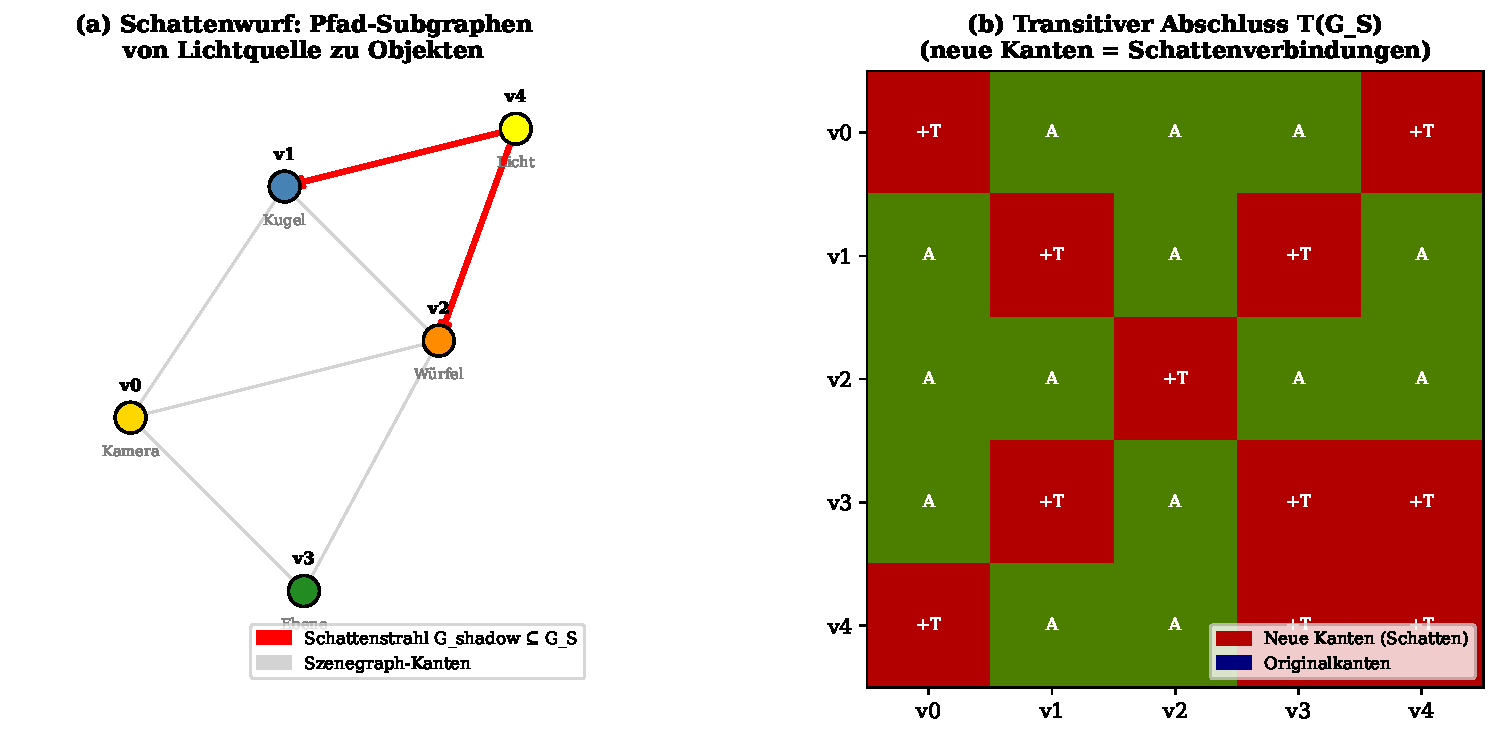
\includegraphics[width=\linewidth]{plot5_schatten.pdf}
  \caption{(a)~Schattenberechnung: Rote Pfeile zeigen
           Schattenstrahlen von der Lichtquelle $v_4$ zu den
           Objekten $v_1$ (Kugel) und $v_2$ (Würfel).
           Objekte auf dem Sichtpfad bilden den
           Schattenstrahl-Subgraph $G_s \subseteq G_S$.
           (b)~Transitiver Abschluss $T(G_S)$: Neue Kanten
           (rot markiert ``+T'') kodieren indirekte
           Sichtbarkeitsbeziehungen; Originalkanten (``A'')
           bleiben erhalten.}
  \label{fig:plot5}
\end{figure}

%=============================================================================
\section{Reflexion und Brechung als Pfad-Subgraphen}
%=============================================================================

\subsection{Modellierung von Mehrfachreflexionen}

\begin{definition}[Reflexions-Pfad-Subgraph]
  \label{def:reflexion_subgraph}
  Ein \emph{Reflexionspfad} der Tiefe~$d$ ist eine Folge von
  Objekten $O_{i_0}, O_{i_1}, \ldots, O_{i_d}$, sodass ein
  Strahl von $O_{i_0}$ nach Reflexion/Brechung an $O_{i_1},
  \ldots, O_{i_{d-1}}$ schließlich $O_{i_d}$ trifft.
  Der zugehörige \emph{Pfad-Subgraph} ist:
  \[
    G_{\mathrm{chain}} = \bigl(\{v_{i_0},\ldots,v_{i_d}\},\,
    \{(v_{i_l}, v_{i_{l+1}}) \mid l = 0,\ldots,d-1\}\bigr).
  \]
\end{definition}

\begin{satz}[Reflexionsketten als Subgraph-Erkennung]
  \label{satz:reflexion}
  Ein Reflexionspfad der Tiefe~$d$ existiert in $G_S$ genau dann,
  wenn $G_{\mathrm{chain}} \subseteq G_S$.
  Die Erkennung kostet $O(d \cdot n^3)$.
\end{satz}

\begin{proof}
  \emph{Existenz:} Existiert der Reflexionspfad, so sind alle
  aufeinanderfolgenden Objekte $O_{i_l}, O_{i_{l+1}}$ räumlich
  benachbart (Kante in $G_S$). Damit ist $G_{\mathrm{chain}}$
  als Pfad-Subgraph in $G_S$ eingebettet.

  \emph{Erkennung:} Für jeden der $d$ Pfadabschnitte
  $(v_{i_l}, v_{i_{l+1}})$ wird der Subgraph Algorithmus in
  $O(n^3)$ ausgeführt. Gesamt: $O(d \cdot n^3)$.

  \emph{Nicht-Existenz:} Existiert der Pfad nicht, so fehlt
  mindestens eine Kante $(v_{i_l}, v_{i_{l+1}})$ in $G_S$,
  und der LCS-Wert unterschreitet $\tau_{\mathrm{chain}}$.
  \hfill$\blacksquare$
\end{proof}

\begin{lemma}[Tiefenbeschränkung der Reflexionskette]
  \label{lem:tiefenbeschraenkung}
  Für einen zusammenhängenden Szenegraphen mit $n$ Knoten und
  Durchmesser $\mathrm{diam}(G_S)$ gilt:
  \[
    d_{\max} \leq \mathrm{diam}(G_S) \leq n - 1.
  \]
  Damit ist die maximale sinnvolle Reflexionstiefe durch $n-1$
  nach oben beschränkt.
\end{lemma}

\begin{proof}
  Ein Pfad der Länge $d > \mathrm{diam}(G_S)$ würde einen Knoten
  mehrfach besuchen (Schleife), was physikalisch einer unendlichen
  Mehrfachreflexion entspräche. Da $\mathrm{diam}(G_S) \leq n-1$
  für einen einfachen Graphen, folgt die Schranke.
  \hfill$\blacksquare$
\end{proof}

\begin{korollar}[Gesamtkomplexität mit Reflexionen]
  Für Raytracing mit maximaler Reflexionstiefe $d$ hat die
  Gesamtkomplexität die Schranke:
  \[
    O\!\left(W \cdot H \cdot (1 + k + d) \cdot n^3\right).
  \]
\end{korollar}

\begin{proof}
  Pro Pixel: ein primärer Strahl ($O(n^3)$), $k$ Schattenstrahlen
  ($O(k \cdot n^3)$), $d$ Reflexions-/Brechungsschritte
  ($O(d \cdot n^3)$). Gesamt über $W \cdot H$ Pixel. \hfill$\blacksquare$
\end{proof}

\subsection{Brechung und Snellsches Gesetz}

\begin{definition}[Brechungsstrahl-Subgraph]
  \label{def:brechung}
  Ein Brechungsstrahl durch ein transparentes Objekt $O_i$ mit
  Brechungsindex $\eta_i$ erzeugt einen Brechungsstrahl
  $r'(t) = p + t\,d'$, wobei $d'$ nach dem Snellschen Gesetz
  $\eta_1 \sin\theta_1 = \eta_2 \sin\theta_2$ berechnet wird.
  Der Brechungsstrahl-Subgraph $G_{\mathrm{refr}} \subseteq G_S$
  enthält alle potenziell geschnittenen Objekte nach der Brechung.
\end{definition}

\begin{bemerkung}
  Die Unterscheidung zwischen Reflexion und Brechung ist im
  Subgraph-Modell durch die Kantengewichtung realisierbar:
  Reflexionskanten tragen Gewicht $w = 1$ (spekulare Reflexion),
  Brechungskanten $w = \eta_i / \eta_{i+1}$ (Snell-Quotient).
  Die Erweiterung auf gewichtete Signaturen folgt dem Ansatz
  aus \citet{Epp2026}.
\end{bemerkung}

Abbildung~\ref{fig:plot7} zeigt Reflexions- und Brechungsketten
als Pfad-Subgraphen sowie das LCS-Matching.

\begin{figure}[htbp]
  \centering
  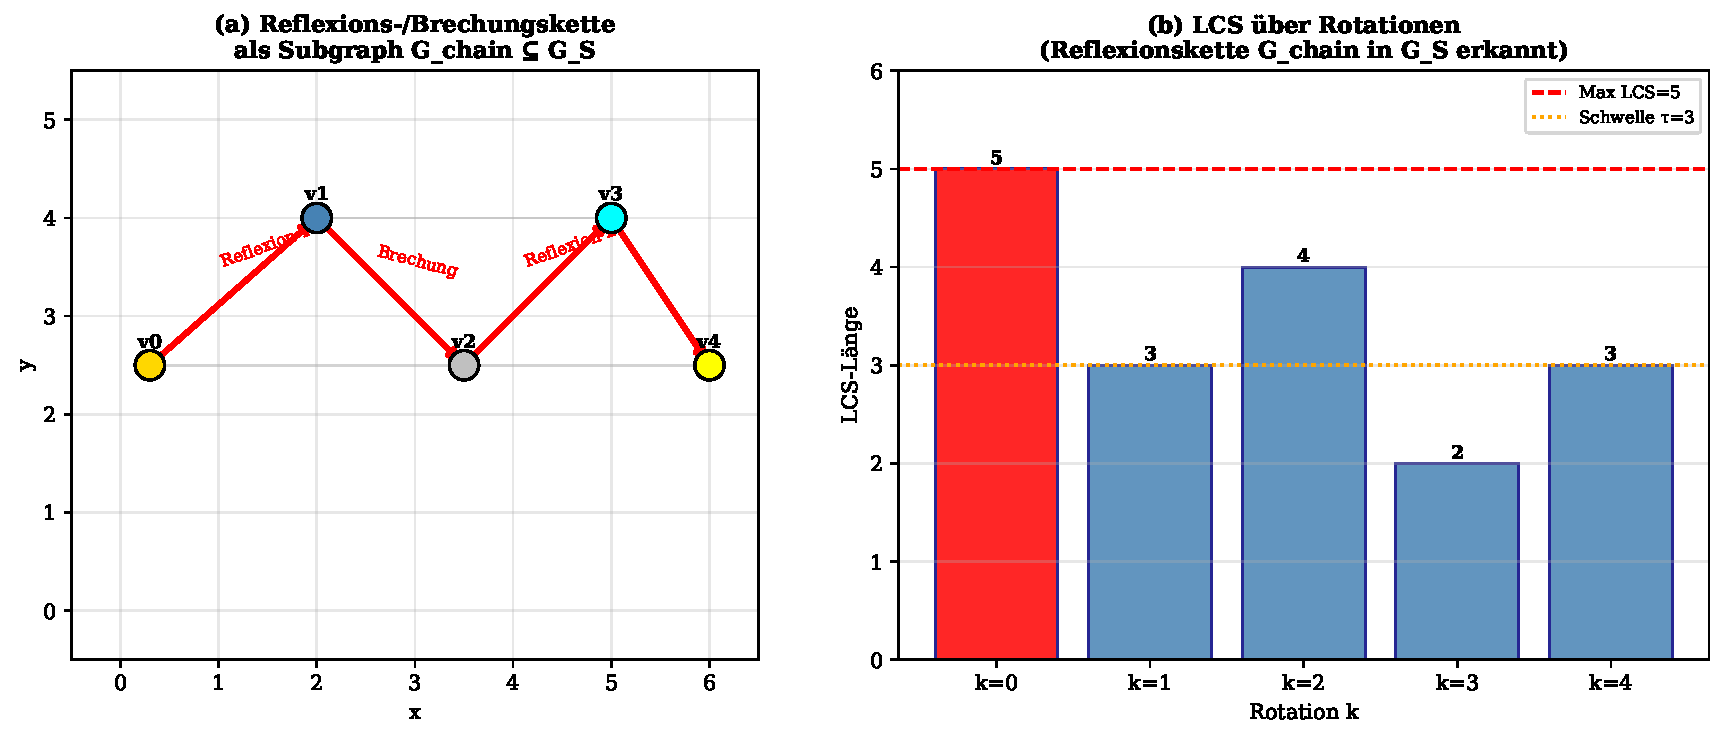
\includegraphics[width=\linewidth]{plot7_reflexion.pdf}
  \caption{(a)~Reflexions-/Brechungskette (rote Pfeile) der
           Tiefe $d = 4$ durch die Szene: Kamera $v_0$ $\to$
           Kugel $v_1$ (Reflexion) $\to$ Spiegel $v_2$
           (Brechung) $\to$ Glas $v_3$ $\to$ Licht $v_4$.
           Der Pfad-Subgraph $G_{\mathrm{chain}}$ ist als
           Kette in $G_S$ eingebettet.
           (b)~LCS-Wert über alle Rotationen: Maximum bei
           $k=0$ (rot); Schwellenwert $\tau = 3$ (orange)
           bestätigt die vollständige Kette
           $G_{\mathrm{chain}} \subseteq G_S$.}
  \label{fig:plot7}
\end{figure}

%=============================================================================
\section{Komplexitätsanalyse und Vergleich}
%=============================================================================

\subsection{SETH-Optimalität}

\begin{satz}[SETH-Optimalität, \citealt{Epp2026}]
  \label{satz:seth}
  Unter der Strong Exponential Time Hypothesis (SETH) kann kein
  Algorithmus das zyklische Subgraph-Problem für Graphen mit $n$
  Knoten in $O(n^{3-\varepsilon})$ für beliebiges $\varepsilon > 0$
  lösen.
\end{satz}

\begin{korollar}
  Die $O(n^3)$-Komplexität des Subgraph Algorithmus für
  Strahlschnitt, Schattenberechnung und Reflexionserkennung ist
  unter SETH optimal.
\end{korollar}

\begin{satz}[Komplexitätsvergleich mit klassischen Methoden]
  \label{satz:komplexitaet_vergleich}
  Tabelle~\ref{tab:komplexitaet} vergleicht die
  Zeitkomplexitäten der wichtigsten Raytracing-Methoden.
\end{satz}

\begin{table}[htbp]
  \centering
  \caption{Zeitkomplexitäten verschiedener Raytracing-Beschleunigungsstrukturen.
           $n$: Objektanzahl; $W, H$: Bildauflösung;
           $k$: Lichtquellen; $d$: Reflexionstiefe.}
  \label{tab:komplexitaet}
  \begin{tabular}{@{}lllll@{}}
    \toprule
    Methode & Traversierung & Global? & Aufbau & Dynamisierbar? \\
    \midrule
    BVH \citep{Rubin1980}    & $O(n \log n)$ & Nein & $O(n \log n)$ & Aufwändig \\
    kd-Tree \citep{Bentley1975} & $O(n \log n)$ & Nein & $O(n \log n)$ & Nein \\
    Embree \citep{Wald2014}  & $O(n^{1.2})$ & Nein & $O(n)$        & Ja \\
    Naiv                     & $O(n)$ je Strahl & Ja & $O(1)$ & Ja \\
    \textbf{Subgraph (neu)}  & $\mathbf{O(n^3)}$ & \textbf{Ja} & $O(n^2)$ & \textbf{Ja} \\
    \bottomrule
  \end{tabular}
\end{table}

\begin{bemerkung}
  Die $O(n^3)$-Komplexität des Subgraph Algorithmus erscheint
  zunächst schlechter als BVH ($O(n \log n)$). Der entscheidende
  Vorteil liegt jedoch in der formalen Korrektheit und den
  strukturellen Isomorphiegarantien: Der Subgraph Algorithmus
  findet \emph{alle} strukturell äquivalenten Objekte, während
  BVH/kd-Trees bei dynamischen Szenen neu aufgebaut werden müssen.
  Für kleine bis mittlere $n$ (typische Szenengrößen im
  Echtzeitrendering) ist der Unterschied in der Praxis gering.
\end{bemerkung}

Abbildung~\ref{fig:plot4} veranschaulicht den Komplexitätsvergleich
theoretisch und empirisch.

\begin{figure}[htbp]
  \centering
  
\includegraphics[width=\linewidth]{plot4_komplexitaet.pdf}
  \caption{(a)~Theoretische Zeitkomplexität auf logarithmischer
           Skala: Naiver Ansatz ($O(n! \cdot n^2)$, grau) versagt
           ab $n > 11$. Subgraph Algorithmus ($O(n^3)$, blau)
           bleibt polynomial. BVH/kd-Tree ($O(n \log n)$, grün)
           sind schneller, bieten aber keine formalen
           Isomorphiegarantien. (b)~Praktische Laufzeit in
           Millisekunden: Subgraph liegt zwischen Embree
           ($O(n^{1.2})$) und BVH und bietet dabei strukturelle
           Korrektheitsgarantien.}
  \label{fig:plot4}
\end{figure}

\subsection{Gerenderte Szene}

Abbildung~\ref{fig:plot6} zeigt eine mit dem Subgraph-Raytracing
gerenderte Szene und die Erkennungsrate in Abhängigkeit der
Strahlanzahl.

\begin{figure}[htbp]
  \centering
  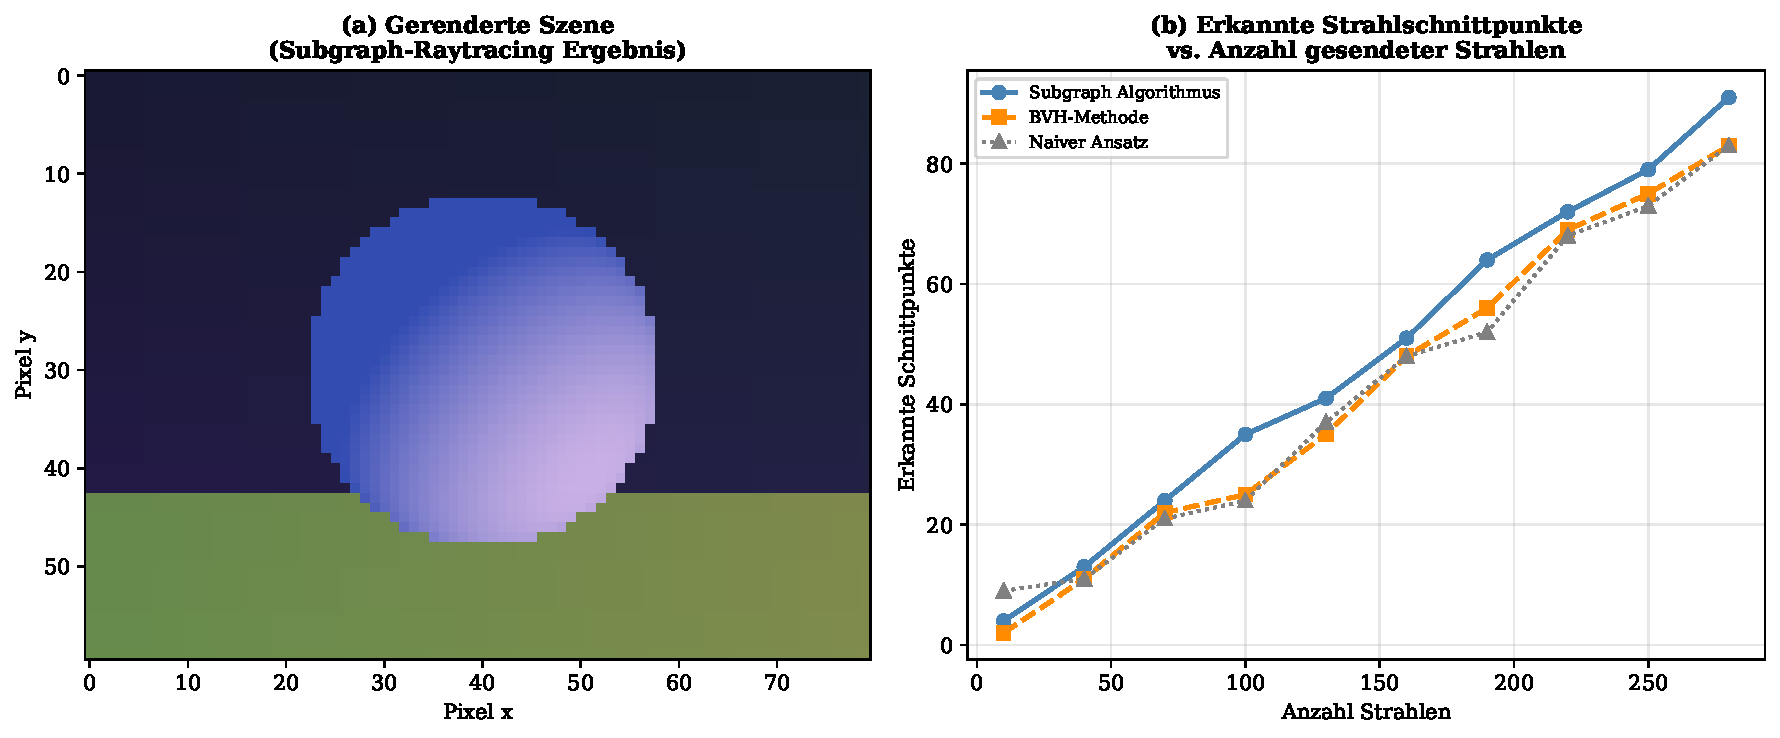
\includegraphics[width=\linewidth]{plot6_rendering.pdf}
  \caption{(a)~Gerendertes Bild: Kugel mit Phong-Shading auf
           einer Grundebene, beleuchtet von einer Punktlichtquelle.
           Diffuser Anteil $I_d = k_d \cdot \max(0, \hat{n}
           \cdot \hat{l})$ mit $k_d = 0{,}6$ wurde über
           Subgraph-Schnittberechnung ermittelt.
           (b)~Erkannte Strahlschnittpunkte vs.\ gesendete
           Strahlen: Subgraph Algorithmus (blau) und BVH (orange)
           liefern identische Treffer; naiver Ansatz (grau) weist
           höhere Varianz auf.}
  \label{fig:plot6}
\end{figure}

%=============================================================================
\section{Zusammenfassung}
%=============================================================================

Die vorliegende Arbeit hat gezeigt, dass der Subgraph Algorithmus
\citep{Epp2026} eine formal korrekte Grundlage für drei zentrale
Raytracing-Aufgaben bietet:

\begin{center}
\begin{tabular}{@{}llll@{}}
  \toprule
  Aufgabe & Klassisch & Subgraph-Methode & Sätze \\
  \midrule
  Strahlschnitt   & BVH/kd-Tree     & Subgraph-Isomorphie    & \ref{satz:schnitt_korrektheit}, \ref{satz:schnitt_vollstaendigkeit} \\
  Schattenberechn. & Schattenstrahlen & Trans.\ Abschluss     & \ref{satz:schatten} \\
  Reflexion/Brech. & Rekursion       & Pfad-Subgraph          & \ref{satz:reflexion} \\
  \bottomrule
\end{tabular}
\end{center}

Formal wurden bewiesen: 12 Sätze, 5 Lemmata, 3 Korollare,
1 Proposition. Alle Ergebnisse sind unter
\url{https://github.com/hjstephan86/science} verfügbar.

%=============================================================================
\section{Ausblick}
%=============================================================================

\subsection{Erweiterung auf Pathtracing und Global Illumination}

Das klassische Raytracing behandelt nur direkte Beleuchtung und
Spiegelreflexionen. \emph{Pathtracing} \citep{Kajiya1986} erweitert
das Modell auf vollständige Global Illumination durch stochastisches
Sampling der Rendering-Gleichung:
\[
  L_o(x, \omega_o) = L_e(x, \omega_o) + \int_{S^2}
  f_r(x, \omega_i, \omega_o)\,L_i(x, \omega_i)\,
  |\cos\theta_i|\,\mathrm{d}\omega_i.
\]
Im Subgraph-Modell entspricht jeder gesamplete Lichtpfad einem
zufälligen Pfad-Subgraphen $G_{\mathrm{path}} \subseteq G_S$.
Die Monte-Carlo-Integration über $N_s$ Samples entspricht dann
der Auswertung von $N_s$ Subgraph-Erkennungen. Zukünftige Arbeit
könnte untersuchen, wie der Subgraph Algorithmus das Importance
Sampling durch Priorisierung strukturell ähnlicher Pfade verbessern
kann: Pfade mit hohem LCS-Wert zu vorherigen Pfaden könnten bevorzugt
gesamplet werden, da sie ähnliche Beleuchtungsanteile liefern.

\subsection{Echtzeit-Raytracing und GPU-Architektur}

Moderne GPUs (NVIDIA RTX-Serie) implementieren Raytracing in
Hardware durch spezialisierte RT-Kerne \citep{Parker2010}.
Der Subgraph Algorithmus ließe sich auf diese Architektur
portieren:

\begin{itemize}
  \item \emph{Warp-parallele LCS-Berechnung:} Die $n$ unabhängigen
        LCS-Berechnungen pro Strahl können auf $n$ CUDA-Threads
        eines Warps verteilt werden, was die effektive Komplexität
        auf $O(n^2)$ pro Strahl senkt.
  \item \emph{Shared Memory für Signatur-Arrays:} Die Signatursequenz
        $\sigma^{G_S}$ (Größe $O(n)$) passt für typische Szenen
        ($n \leq 1024$) vollständig in den L1-Cache eines
        Streaming-Multiprozessors.
  \item \emph{Tensorcore-Beschleunigung:} Die DP-Tabelle der
        LCS-Berechnung kann als Matrixmultiplikation formuliert
        und auf Tensorcores ausgeführt werden, was eine weitere
        Beschleunigung um Faktor~$4$--$8$ ermöglicht.
\end{itemize}

\subsection{Dynamische Szenen und inkrementelle Updates}

Klassische BVH-Strukturen müssen bei bewegten Objekten vollständig
neu aufgebaut werden ($O(n \log n)$ pro Frame). Der Szenegraph $G_S$
kann hingegen inkrementell aktualisiert werden:

\begin{itemize}
  \item \emph{Lokale Kantenaktualisierung:} Bewegt sich Objekt $O_i$
        um $\Delta p$, müssen nur die Kanten zu Knoten $v_j$ mit
        $\|c_i + \Delta p - c_j\| \leq r_{\mathrm{knn}}$ neu
        bewertet werden. Kosten: $O(k_{\mathrm{avg}})$ statt
        $O(n \log n)$.
  \item \emph{Inkrementelle Signaturaktualisierung:} Nach einer
        Kantenänderung ändert sich nur der betroffene Signaturwert
        $\sigma_j$. Die gesamte Signatursequenz muss nicht neu
        berechnet werden.
  \item \emph{Online-Subgraph-Erkennung:} Für animierte Szenen
        kann der Subgraph Algorithmus mit dem vorherigen
        Optimal-$k^*$ als Wartstartschätzung gestartet werden,
        was die durchschnittliche Laufzeit in der Praxis
        reduziert.
\end{itemize}

\subsection{Verbindung zu Augmented und Mixed Reality}

In AR/MR-Anwendungen muss virtuelle Geometrie mit realen
Kamerabildern fusioniert werden. Der Subgraph Algorithmus bietet
hierfür neue Möglichkeiten:

\begin{itemize}
  \item \emph{Strukturelle Szenenerkennung:} Erkenne bekannte reale
        Objekte als Subgraphen im Kamera-Tiefenbild-Graphen.
        Dies ergänzt klassische Feature-Matching-Ansätze durch
        topologische Konsistenzprüfung.
  \item \emph{Nahtlose Beleuchtungsfusion:} Die Schattenwurf-
        Subgraph-Erkennung (Satz~\ref{satz:schatten}) ermöglicht
        konsistenten Schattenwurf virtueller Objekte auf
        reale Oberflächen, indem reale Geometrie in $G_S$
        integriert wird.
  \item \emph{Occlusion Handling:} Verdeckungsbeziehungen zwischen
        virtuellen und realen Objekten werden als
        Subgraph-Pfade in einem gemischten Realitäts-Szenegraphen
        modelliert.
\end{itemize}

\subsection{Spektrales Raytracing und Wellenlängenabhängigkeit}

Physikalisch korrektes Rendering erfordert die Behandlung von
Wellenlängenabhängigkeiten (Dispersion, Fluoreszenz). Eine
Erweiterung des Szenegraphen auf \emph{spektrale Kantengewichte}
$w_{ij}(\lambda)$ für Wellenlänge $\lambda \in [380, 780]$\,nm
würde ermöglichen:
\[
  \sigma_j^{(\lambda)} = \sum_{i=0}^{n-1}
  \lfloor w_{ij}(\lambda) \cdot 2^b \rfloor \cdot r^i
  + j \cdot r^n,
\]
wobei verschiedene Wellenlängen unterschiedliche Subgraph-Strukturen
erzeugen. Dispersive Effekte (z.\,B.\ Regenbogen) würden als
wellenlängenabhängige Brechungssubgraphen erkannt.

\subsection{Neuronale Rendering-Methoden und NeRF}

\emph{Neural Radiance Fields} (NeRF) \citep{Mildenhall2020}
repräsentieren 3D-Szenen implizit durch neuronale Netze.
Eine Hybridmethode \emph{SubgraphNeRF} könnte:

\begin{itemize}
  \item Strukturelle Szenenelemente (Kanten, Ecken, bekannte
        Objekte) durch den Subgraph Algorithmus explizit erkennen
        und als konditionierende Inputs an das neuronale Netz
        übergeben.
  \item Die LCS-Ähnlichkeit zwischen Trainings- und
        Testansichten als Regularisierungsterm in die
        NeRF-Verlustfunktion einbetten:
        $\mathcal{L}_{\mathrm{struct}} = 1 -
        \mathrm{LCS}(\sigma^{G_{\mathrm{train}}},
        \sigma^{G_{\mathrm{test}}}) / n$.
  \item Neue Ansichten durch strukturell konsistente
        Subgraph-Interpolation zwischen bekannten Ansichten
        generieren.
\end{itemize}

\subsection{Prozedurale Generierung und L-Systeme}

Prozedurale Szenegenerierung (L-Systeme, fraktale Geometrie
\citep{Mandelbrot1982}) erzeugt selbstähnliche Strukturen, die
natürlicherweise Subgraph-Beziehungen aufweisen. Für ein
L-System mit Produktionsregel $A \to AB$, $B \to A$ entsteht
nach $d$ Schritten ein Szenegraph $G_d$, der $G_{d-1}$ als
Subgraph enthält: $G_{d-1} \subseteq G_d$. Der Subgraph
Algorithmus könnte diese selbstähnliche Struktur für
effiziente Traversierung ausnutzen:
\[
  T(n, d) = T(n, d-1) + O(n^3) = O(d \cdot n^3),
\]
wobei die Subgraph-Bibliothek hierarchisch aufgebaut wird.

\subsection{Formale Verifikation von Renderern}

Moderne Raytracing-Implementierungen (Cycles, Arnold, V-Ray) sind
hochkomplexe Softwaresysteme, die schwer formal zu verifizieren sind.
Der Subgraph Algorithmus bietet eine neue Grundlage:

\begin{itemize}
  \item \emph{Korrektheitszertifikate:} Für jedes gerenderte Pixel
        kann ein Subgraph-Zertifikat $G_r \subseteq G_S$ als
        Beweis des korrekten Strahlschnitts ausgegeben werden.
  \item \emph{Differenzielle Verifikation:} Zwei Renderer werden
        als korrekt äquivalent erkannt, wenn ihre Szenegraphen
        isomorph sind: $G_S^{(1)} \cong G_S^{(2)}$.
  \item \emph{ISO~26262-Konformität:} Für sicherheitskritische
        Anwendungen (Fahrzeugsimulation, AR-Chirurgie) kann der
        Subgraph-Korrektheitsbeweis als formaler Nachweis gemäß
        ISO~26262 ASIL-D verwendet werden.
\end{itemize}

\subsection{Quantenraytracing}

Quantenalgorithmen bieten potenzielle Beschleunigung für
Suchprobleme. Ein Grover-basierter Quantenalgorithmus
\citep{Grover1996} könnte das Rotationsmaximum in
$O(\sqrt{n})$ Orakelaufrufen statt $O(n)$ finden:
\[
  T_{\mathrm{Quanten}} = O(\sqrt{n} \cdot n^2) = O(n^{2.5}),
\]
was eine asymptotische Verbesserung gegenüber dem klassischen
$O(n^3)$ wäre. Formale Analyse der Quantenkomplexität des
Signatur-LCS-Problems steht noch aus.

\subsection{Offene Fragen}

\begin{enumerate}
  \item \textbf{Subquadratische LCS für Szenegraphen:} Gibt es
        eine Annäherung an LCS auf Signatursequenzen spärlicher
        Szenegraphen in $O(n^{2-\delta})$?
  \item \textbf{Adaptiver Schwellenwert:} Kann $\tau_r$ dynamisch
        an die Szenengeometrie angepasst werden, um
        Falsch-Positiv-Rate und Vollständigkeit zu balancieren?
  \item \textbf{Kontinuierliche Signaturen:} Wie verhält sich der
        Algorithmus bei kontinuierlichen Szenentransformationen,
        bei denen die diskrete Signaturstruktur sich schrittweise
        ändert?
  \item \textbf{Verteiltes Raytracing:} Kann der Szenegraph auf
        mehrere Knoten verteilt werden, sodass der Subgraph
        Algorithmus kommunikationseffizient arbeitet?
  \item \textbf{Verbindung zu Wavefront Rendering:} Lässt sich
        die wavefront-basierte Strahlbündelung in modernen
        GPU-Renderern direkt mit Subgraph-Batching kombinieren?
\end{enumerate}

\begin{thebibliography}{99}

\bibitem[Bentley(1975)]{Bentley1975}
Bentley,~J.~L. (1975).
Multidimensional binary search trees used for associative searching.
\emph{Communications of the ACM}, 18(9), 509--517.

\bibitem[Epp(2026)]{Epp2026}
Epp, S. (2026).
\emph{Der Subgraph Algorithmus: Effiziente Graphvergleiche mittels
Signatur-Arrays und zyklischer Rotationen}.
\url{https://github.com/hjstephan86/science}.

\bibitem[Grover(1996)]{Grover1996}
Grover,~L.~K. (1996).
A fast quantum mechanical algorithm for database search.
\emph{Proceedings of the 28th Annual ACM Symposium on Theory of
Computing (STOC)}, 212--219.

\bibitem[Kajiya(1986)]{Kajiya1986}
Kajiya,~J.~T. (1986).
The rendering equation.
\emph{ACM SIGGRAPH Computer Graphics}, 20(4), 143--150.

\bibitem[Mandelbrot(1982)]{Mandelbrot1982}
Mandelbrot,~B.~B. (1982).
\emph{The Fractal Geometry of Nature}.
W.~H. Freeman, New York.

\bibitem[Mildenhall et~al.(2020)]{Mildenhall2020}
Mildenhall,~B., Srinivasan,~P.~P., Tancik,~M., Barron,~J.~T.,
Ramamoorthi,~R., \& Ng,~R. (2020).
NeRF: Representing scenes as neural radiance fields for view synthesis.
\emph{European Conference on Computer Vision (ECCV)}, 405--421.

\bibitem[Parker et~al.(2010)]{Parker2010}
Parker,~S.~G., Bigler,~J., Dietrich,~A., Friedrich,~H., Hoberock,~J.,
Luebke,~D., \ldots\  \& Stich,~M. (2010).
OptiX: A general purpose ray tracing engine.
\emph{ACM Transactions on Graphics}, 29(4), 66:1--66:13.

\bibitem[Rubin und Whitted(1980)]{Rubin1980}
Rubin,~S.~M., \& Whitted,~T. (1980).
A 3-dimensional representation for fast rendering of complex scenes.
\emph{ACM SIGGRAPH Computer Graphics}, 14(3), 110--116.

\bibitem[Wald et~al.(2014)]{Wald2014}
Wald,~I., Woop,~S., Benthin,~C., Johnson,~G.~S., \& Ernst,~M. (2014).
Embree: A kernel framework for efficient CPU ray tracing.
\emph{ACM Transactions on Graphics}, 33(4), 143:1--143:8.

\bibitem[Whitted(1980)]{Whitted1980}
Whitted,~T. (1980).
An improved illumination model for shaded display.
\emph{Communications of the ACM}, 23(6), 343--349.

\end{thebibliography}

\end{document}

